\documentclass[a4paper]{article}
\usepackage[warn]{mathtext} %для поддержки кириллицы в формулах
\usepackage{amsmath} %основной пакет для формул
\usepackage[utf8x]{inputenc}
\usepackage[T1,T2A]{fontenc}
\usepackage[russian]{babel}
\usepackage{hyperref}
\usepackage{indentfirst}
\usepackage{listings}
\usepackage{color}
\usepackage{xcolor}
\usepackage{here}
\usepackage{array}
\usepackage{multirow}
\usepackage{graphicx}

\definecolor{linkcolor}{HTML}{000000} % цвет ссылок 000000 = чёрный
\definecolor{urlcolor}{HTML}{0000FF} % цвет гиперссылок 0000FF = синий
 
\hypersetup{pdfstartview=FitH, pagecolor=black, linkcolor=linkcolor,urlcolor=urlcolor, colorlinks=true}
\usepackage{caption}

\renewcommand{\lstlistingname}{Программа} % заголовок листингов кода

\usepackage{listings}
\lstset{ %
extendedchars=\true,
keepspaces=true,
language=c++,					% choose the language of the code
basicstyle=\footnotesize,		% the size of the fonts that are used for the code
numbers=left,					% where to put the line-numbers
numberstyle=\footnotesize,		% the size of the fonts that are used for the line-numbers
stepnumber=1,					% the step between two line-numbers. If it is 1 each line will be numbered
numbersep=5pt,					% how far the line-numbers are from the code
backgroundcolor=\color{white},	% choose the background color. You must add \usepackage{color}
showspaces=false				% show spaces adding particular underscores
showstringspaces=false,			% underline spaces within strings
showtabs=false,					% show tabs within strings adding particular underscores
frame=single,           		% adds a frame around the code
tabsize=2,						% sets default tabsize to 2 spaces
captionpos=b,					% sets the caption-position to bottom
breaklines=true,				% sets automatic line breaking
breakatwhitespace=false,		% sets if automatic breaks should only happen at whitespace
escapeinside={\%*}{*)},			% if you want to add a comment within your code
postbreak=\raisebox{0ex}[0ex][0ex]{\ensuremath{\color{red}\hookrightarrow\space}}
}

\usepackage[left=2cm,right=2cm,
top=2cm,bottom=2cm,bindingoffset=0cm]{geometry}


\begin{document}	% начало документа

\begin{titlepage}	% начало титульной страницы

	\begin{center}		% выравнивание по центру

		\large Санкт-Петербургский Политехнический Университет Петра Великого\\
		\large Институт компьютерных наук и технологий \\
		\large Кафедра компьютерных систем и программных технологий\\[2cm]
		% название института, затем отступ 6см
		
		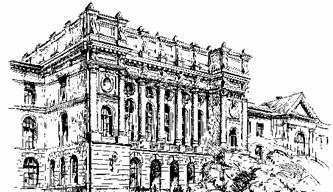
\includegraphics[scale=0.7]{pics/spbpu.jpg}\\[2cm]		
		
		\huge Название предмета\\[0.5cm] % название работы, затем отступ 0,5см
		\large Отчет по лабораторной работе №1\\[0.1cm]
		\large Тема работы\\[5cm]

	\end{center}


	\begin{flushright} % выравнивание по правому краю
		\begin{minipage}{0.25\textwidth} % врезка в половину ширины текста
			\begin{flushleft} % выровнять её содержимое по левому краю

				\large\textbf{Работу выполнил:}\\
				\large Петров В.Д.\\
				\large {Группа:} 43501/4\\
				
				\large \textbf{Преподаватель:}\\
				\large Ицыксон В.М.

			\end{flushleft}
		\end{minipage}
	\end{flushright}
	
	\vfill % заполнить всё доступное ниже пространство

	\begin{center}
	\large Санкт-Петербург\\
	\large \the\year % вывести дату
	\end{center} % закончить выравнивание по центру

\thispagestyle{empty} % не нумеровать страницу
\end{titlepage} % конец титульной страницы

\vfill % заполнить всё доступное ниже пространство



% Содержание
\hypertarget{toc}
\tableofcontents
\newpage

%TODO

\section*{Игра Го}
\addcontentsline{toc}{section}{Глава 1. Игра Го}

%Глава -- Описание предметной области (должно называться типа "Японская игра Сеги", "Эмулятор звездной системы", "Модель хищник-жертва" и %т. п.). Там размещаем то, что есть в ваших репозиториях в README.md, кроме диаграммы компонентов.\\

\subsection*{Задание}
  Разработать приложение для игры Го.\\

\subsection*{Правила игры}

\subsubsection*{Основная часть}
\begin{itemize}

\item Го представляет собой доску размера $19 \times 19$ пунктов (пересечений прямых линий) и камни двух цветов: чёрные и белые. В Го задействованы 2 игрока, один из которых играет чёрными камнями, а другой - белыми. Распределение игровых цветов между соперниками происходит в соответствии с процедурой нигири. Изначально доска пуста. Правом первого хода обладает игрок, которому достались чёрные камни. Далее игроки до завершения игры поочерёдно делают ходы. Засчёт того, что чёрные обладают правом первого хода, белым дается компенсация ввиде коми - определённого нецелого числа очков.\\

\item Процедура нигири подразумевает следующее: один игрок берет в руку горсть белых камней так, чтобы соперник не видел их количество. Другой берет один или два чёрных камня, тем самым пытаясь угадать соответственно чётность или нечётность количества белых камней. Затем игроки выкладывают камни на доску. Если второй игрок угадал чётность, то он играет чёрными, а в противном случае - белыми.\\

\item Ход заключается в том, что игрок пассует (пропускает ход) или устанавливает камень своего цвета в любой свободный пункт на доске, если это не противоречит двум правилам:
  \begin{enumerate}
  
  \item Устанавливаемый камень должен иметь хотя бы одно дыхание. Дыханием называется свободный соседний пункт, соединенный с данным камнем по прямой линии. Тем не менее, ход может быть осуществлен так, что устанавливаемый камень лишает свою группу дыхания, но при этом лишает дыхания еще и группу соперника, тем самым съедая её.\\
 
  \item  Данный ход игрока не повторяет его предыдущий ход.\\
  
  \end{enumerate}

\item Съедение группы камней (или одного камня) соперника считается осуществлённым, если эта группа камней не имеет
    ни одного дыхания, то есть ни один камень группы не имеет дыханий. Съеденные камни снимаются с доски и остаются до
    конца игры у "съевшего" их игрока.\\
    
\item Цель игроков - к концу игры набрать больше очков, чем соперник. Очко даётся за каждый пункт захваченной территории и, в зависимости от правил, за съеденный или захваченный камень соперника или свой живой камень. Территория считается захваченной игроком, если при максимально эффективной игре обоих игроков он сможет съесть или захватить все камни соперника на данной территории. Захваченный камень - это камень соперника, который имеет дыхания, но при желании игрока может быть съеден.\\

\item Игра завершается в трёх случаях:


\begin{enumerate}

	\item Один из игроков сдается.\\
	\item В ответ на пропуск хода одним игроком следует пропуск хода другим.\\
	\item  Не осталось ходов, способных повлиять на ситуацию на доске.\\

\end{enumerate}

\item Все разыгрываемые в партии очки - целые. Поэтому, с учётом того, что коми - нецелое число, победитель определяется всегда.\\

\end{itemize}

\subsubsection*{Особенности японских правил}

\begin{enumerate}

\item Коми составляет 6,5 очков.\\
\item Способ подсчета очков: размер территории + количество захваченных камней противника, включая съеденные камни + коми (для белых).

\end{enumerate}

\subsubsection*{Особенности китайских правил}

\begin{enumerate}

\item Коми составляет 7,5 очков.\\
\item Способ подсчета очков: размер территории + количество своих живых камней (то есть камней, выставленных на доску и не взятых противником) + коми (для белых).\\

\end{enumerate}
 
\subsection*{Концепция}

  Готовый продукт является кроссплатформенным и содержит приложение как консольное, так и с графическим интерфесом. Есть искусственный интеллект (ИИ), который обладает простой логикой, а не случайно ходит в свободный пункт. Имеется возможность выбрать правила игры: японские или китайские. Определенный правилами размер игровой доски $19 \times 19$ пунктов можно изменить на $13 \times 13$ и $7 \times 7$. Наличие ИИ позволяет не только играть двоим пользователям друг против друга, но и играть одному пользователю против ИИ. Выбор цвета камней происходит либо по договоренности (в случае игры против ИИ цвет выбирает пользователь), либо в соответствии с реализованной традиционной процедурой нигири. Ход событий текущей партии можно сохранить и в дальнейшем - загрузить и продолжить. Пользовательский интерфейс включает справочную систему как по самому интерфейсу, так и по игровому процессу.
  
  Разработка сопровождается модульным и функциональным тестированием на всех этапах.

\subsection*{Минимально работоспособный продукт}

 Кроссплатформеное консольное приложение, позволяющее совершать ходы двоим пользователям.
  
\subsection*{Диаграммы вариантов использования}

\begin{figure}[H]
	\begin{center}
		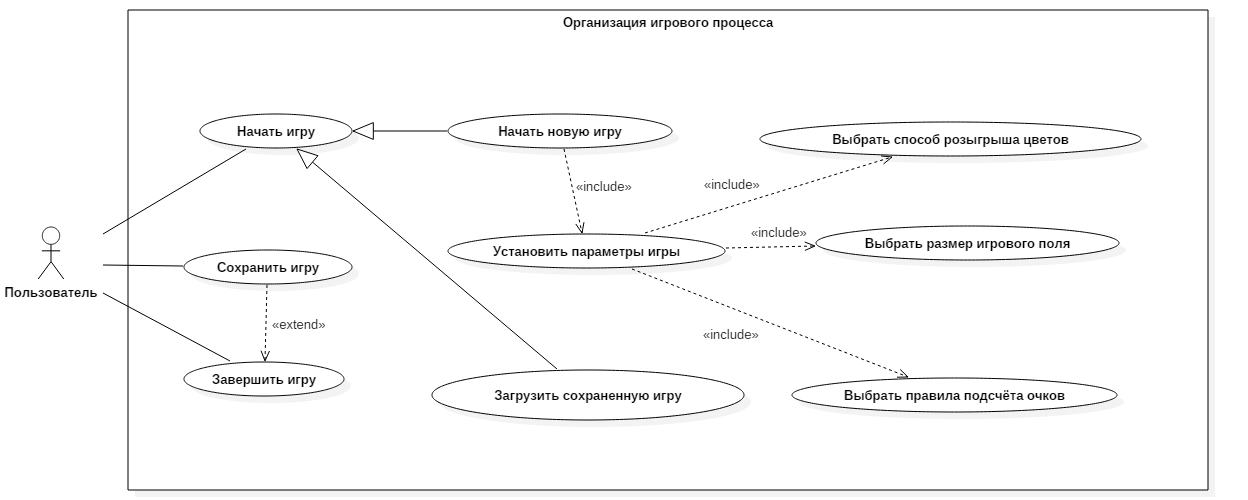
\includegraphics[scale=0.65]{../UMLdiagrams/UseCase/GameOrganisation.png}
		%\caption{название картинки} 
		\label{pic:GameOrganisation}
	\end{center}
\end{figure}

\begin{figure}[H]
	\begin{center}
		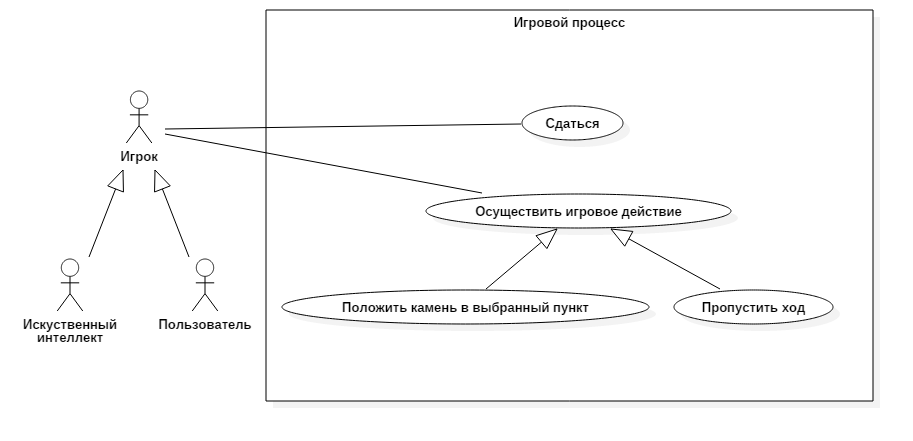
\includegraphics[scale=0.545]{../UMLdiagrams/UseCase/GameProcess.png}
		%\caption{название картинки} 
		\label{pic:GameProcess}
	\end{center}
\end{figure}

\section*{Проектирование приложения, реализующего игру Го}
\addcontentsline{toc}{section}{Глава 2. Проектирование приложения, реализующего эмулятор игры Го}

%Глава -- Проектирование ("Проектирование приложения, реализующего эмулятор звездной системы/японскую игру сеги/модель хищник-жертва". %Здесь описываете архитектуру приложения -- сколько каких подпроектов (какие библиотеки, приложения, тесты), диаграмма компонентов, %описание выделенных интерфейсов (API) человеческим языком, дополнительных библиотек (если использовали), версии языка, кьюти, %компилятора. Описать структуру файлов, если какие-то создаются в процессе работы приложения.\\

В ходе проектирования было принято решение выделить 6 подпроектов: движок - \textbf{GoEngine}, тесты - \textbf{GoTests}, база данных - \textbf{GoDatabase}, 
искусственный интеллект - \textbf{XiGo}, консольное приложение - \textbf{GoCUI} и приложение с графическим интерфейсом - \textbf{GoGUI}. 

\begin{figure}[H]
	\begin{center}
		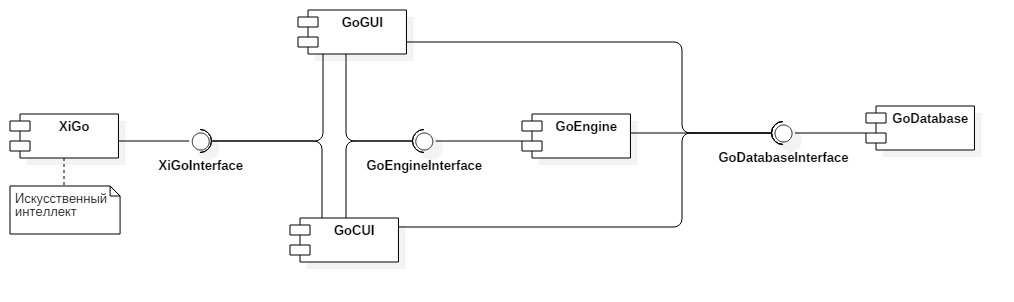
\includegraphics[scale=0.49]{../UMLdiagrams/Component/Component.png}
		%\caption{название картинки} 
		\label{pic:Component}
	\end{center}
\end{figure}

\subsection*{GoEngine}

Подпроект \textbf{GoEngine} - это библиотека, реализующая бизнес-логику игры Го.

\subsubsection*{GoEngine API}

Интерфейс программирования приложения.\\

\begin{itemize}

\item\textbf{void startGame(const int diagonal, const int rules, const int colorDistribution) noexcept override}\\
	
	Создает все объекты, необходимые для игрового процесса. Длина диагонали, правила подсчета очков и способ распределения цветов задаются
	соответственно из параметров diagonal, rules, colorDistribution.\\

\item\textbf{void putStone(const int first, const int second) override}\\
	
	Устанавливает камень игрока, чей ход, в пункт с парой координат (first, second).\\


\item\textbf{void pass() noexcept override}\\

	Устанавливает пропуск хода игроком.\\

\item\textbf{void surrender() noexcept override}\\

	Повзоляет сдаться игроку, чей ход.\\

\item\textbf{Status whoseMove() const noexcept override}\\

	Определяет, чей ход.\\

\item\textbf{bool isGameOver() const noexcept override}\\

	Определяет, окончена ли игра.\\

\item\textbf{Status whoSurrendered() const noexcept override}\\

	Определяет цвет сдавшегося игрока.\\

\item\textbf{Status whoWon() const noexcept override}\\

	Определяет цвет победившего игрока.\\

\item\textbf{int getDiagonal() const noexcept override}\\

	Возвращает значение диагонали доски.\\

\item\textbf{Status getPointsStatus(const int first, const int second) const noexcept override}\\
	
	Определяет статус пункта доски с парой координат (first, second).\\

\item\textbf{int getStonesEatenByBlack() const noexcept override}\\

	Возвращает число съеденных чёрными камней.\\

\item\textbf{int getStonesEatenByWhite() const noexcept override}\\

	Возвращает число съеденных белыми камней.\\

\item\textbf{int getMoveIndex() const noexcept override}\\

	Определяет индекс текущего хода.\\

\item\textbf{std::vector<Move> \&getMoves() const noexcept override}\\

	Возвращает вектор, содержащий ходы.\\

\item\textbf{Move \&getLastMove() const noexcept override}\\

	Возвращает последний совершённый ход.\\

\item\textbf{Move \&getPenultMove() const noexcept override}\\

	Возвращает предпоследний совершённый ход.\\

\item\textbf{int getBlackScore() const noexcept override}\\

	Определяет число очков чёрного игрока.\\

\item\textbf{int getWhiteScore() const noexcept override}\\	

	Определяет число очков белого игрока.\\

\end{itemize}

\subsection*{GoTests}

Подпроект GoTests включает два подпроекта: модульные тесты - \textbf{UnitTests} и функциональные - \textbf{FunctionalTest}.\\

\subsubsection*{UnitTests}
Данный подпроект содержит 5 классов - модульные тесты для 5 классов соответственно из движка GoEngine, которые несут основную функциональную нагрузку:

\begin{itemize}
	\item StoneTest\\
	\item PointTest\\
	\item BoardTest\\
	\item MoveTest\\
	\item GameProcessTest\\
\end{itemize}

\subsubsection*{FunctionalTest}
Данный подпроект содержит 1 класс - \textbf{functionalTest}, задача которого - функциональное тестирование движка \textbf{GoEngine}. В данном классе происходила проверка функиональностей, которые в дальнейшем включались в приложение.

\subsection*{GoDatabase}

База данных, необходимая для загрузки и сохранения процесса игры приложения.\\

\section*{Реализация игры Го}
\addcontentsline{toc}{section}{Глава 3. Реализация игры Го}

%Глава -- Реализация ("Реализация японской игры сеги/модели хищник-жертва"). Здесь описываете среду разработки (версии всех использованых %ос, компиляторов, сред, утилит (qt creator, doxygen, прочее)), очень поверхностно описываете, какие основные классы выделили в каждом из %проектов, если какие-то интересные паттерны или алгоритмы -- тоже. Можно тут рассказать, сколько строк кода. Приводите скрины основных %%экранов пользовательского интерфейса, но чтоб не только картинки, но еще и слова, описывающие то, что видно на картинке. К картинкам не %забывайте делать подписи.

\subsection*{Среда разработки}
\noindent\textbf{Операционная система:} Windows 10.0.10586\\
\textbf{Интегрированная среда разработки:} CLion 2016.1.2\\
\textbf{Стандарт с++:} c++11\\
\textbf{Компилятор:} MinGW 3.21\\
\textbf{Фреймворк для gui:} Qt 5.6\\
\textbf{Система автоматизации сборки:} CMake 3.5.1\\
\textbf{Система документирования:} Doxygen 1.8.11\\
\textbf{Утилита для подсчёта строк:} cloc 1.66\\

\subsection*{GoEngine}

Было выделено 13 классов. Из них 2 относятся к интерфейсу движка, 2 - к правилам игры, 3 - к игровой модели и 6 - к исключениям. Утилитой cloc было посчитано, что в GoEngine 568 строк кода на c++.

\subsection*{GoDatabase}

Не реализовано на данный момент.\\

\subsection*{GoCUI}

Было выделено 2 класса. Один из них, Help, реализует систему помощи. Другой - GoGame - реализует игровой процесс. Утилитой cloc было посчитано, что в GoCUI 792 строк c++-го кода. Данное приложение находится в состоянии mvp.

\begin{figure}[H]
	\begin{center}
		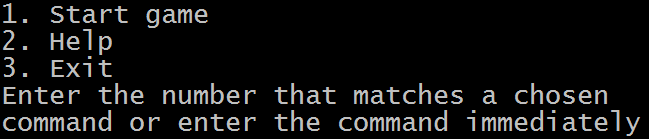
\includegraphics[scale=0.6]{pics/GoCUI/Menu.png}
	    \caption{Главное меню} 
		\label{pic:CUI_Menu}
	\end{center}
\end{figure}

\begin{figure}[H]
	\begin{center}
		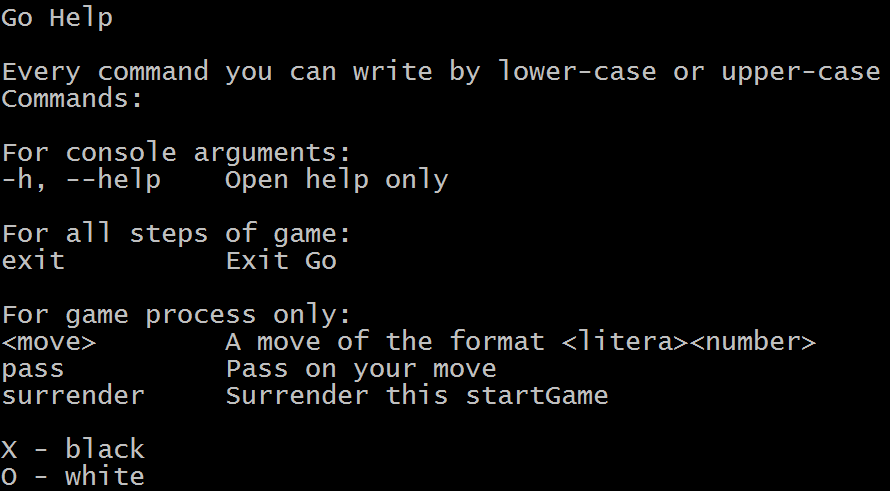
\includegraphics[scale=0.6]{pics/GoCUI/Help.png}
	    \caption{Помощь} 
		\label{pic:CUI_Help}
	\end{center}
\end{figure}

\begin{figure}[H]
	\begin{center}
		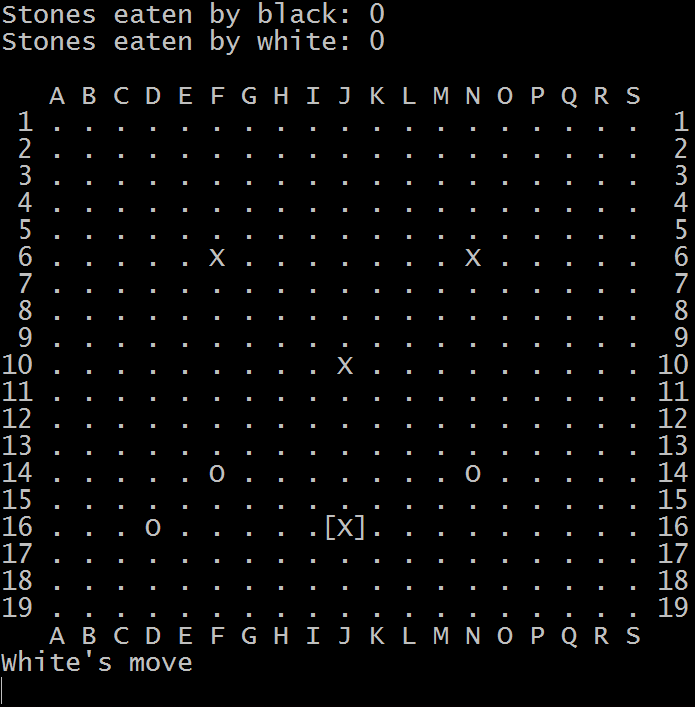
\includegraphics[scale=0.6]{pics/GoCUI/Process.png}
	    \caption{Игровой процесс} 
		\label{pic:CUI_Process}
	\end{center}
\end{figure}

\begin{figure}[H]
	\begin{center}
		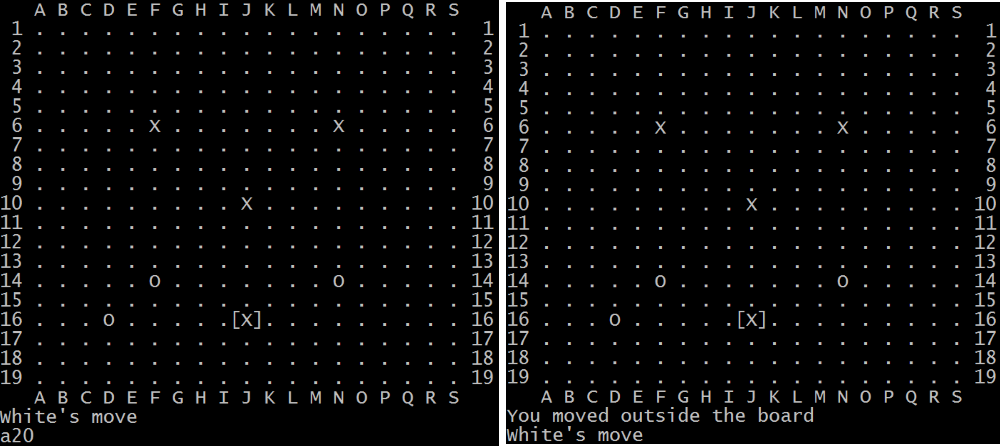
\includegraphics[scale=0.6]{pics/GoCUI/Out.png}
	    \caption{Предупреждение о выходе за границы доски} 
		\label{pic:CUI_Out}
	\end{center}
\end{figure}

\begin{figure}[H]
	\begin{center}
		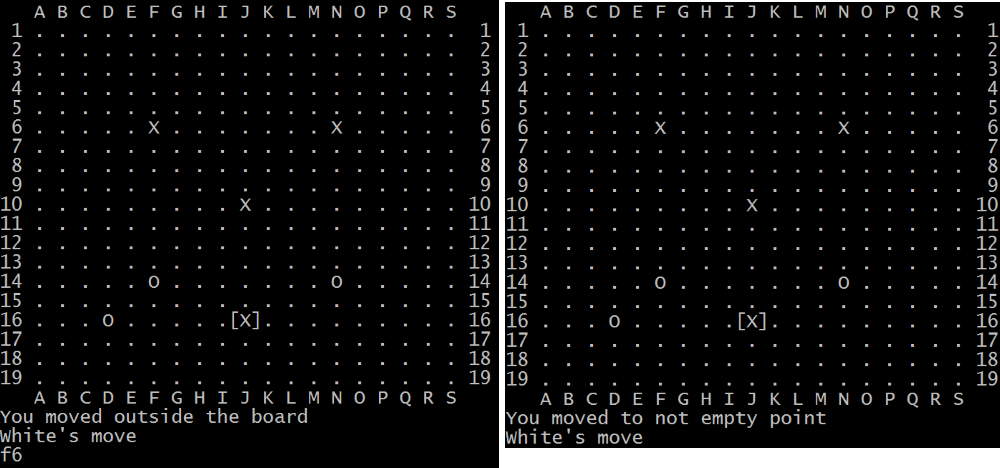
\includegraphics[scale=0.6]{pics/GoCUI/NotEmpty.png}
	    \caption{Предупреждение о ходе в несвободный пункт} 
		\label{pic:CUI_NotEmpty}
	\end{center}
\end{figure}

\begin{figure}[H]
	\begin{center}
		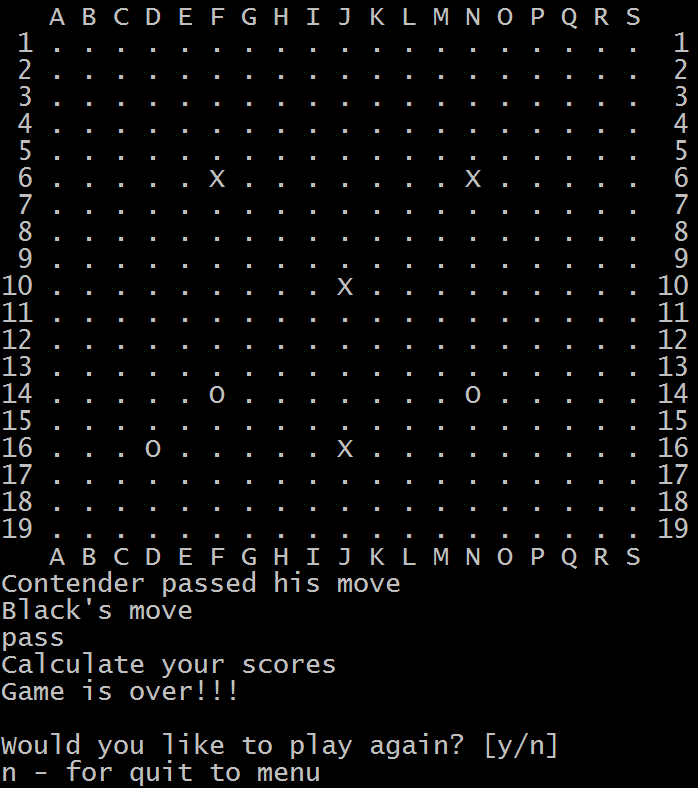
\includegraphics[scale=0.6]{pics/GoCUI/Pass.png}
	    \caption{Предупреждение о пропуске соперником хода и завершение игры после двух попусков подряд} 
		\label{pic:CUI_Pass}
	\end{center}
\end{figure}

\begin{figure}[H]
	\begin{center}
		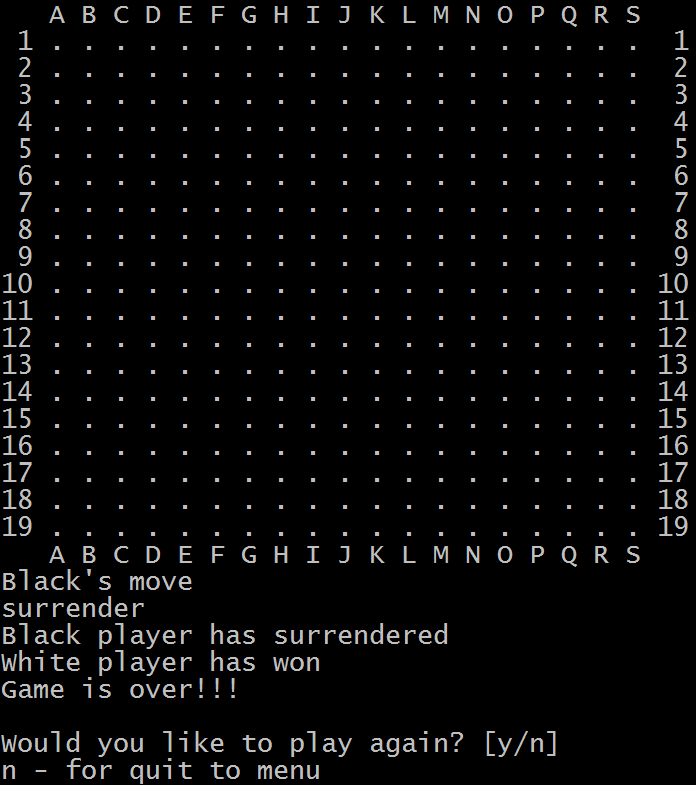
\includegraphics[scale=0.6]{pics/GoCUI/Surrender.png}
	    \caption{Чёрный игрок сдался} 
		\label{pic:CUI_Surrender}
	\end{center}
\end{figure}

\subsection*{GoGUI}

В приложении реализовано на данный момент: окно меню, окно настроек и окно игрового процесса без доски, но с работающими кнопками,
влиющими на игровой процесс. Есть интернационализация.

\begin{figure}[H]
	\begin{center}
		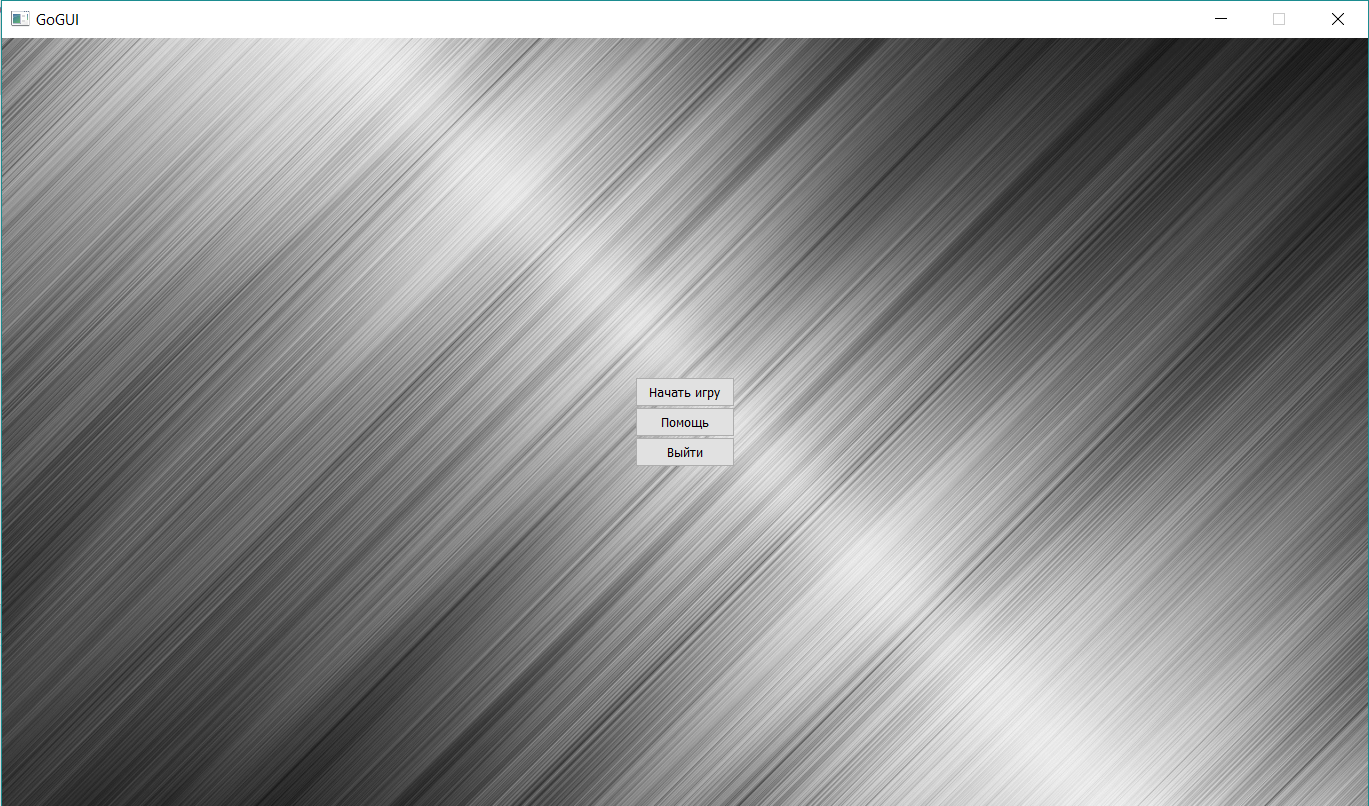
\includegraphics[scale=0.5]{pics/GoGUI/Menu.png}
	    \caption{Главное меню} 
		\label{pic:CUI_Menu}
	\end{center}
\end{figure}

\begin{figure}[H]
	\begin{center}
		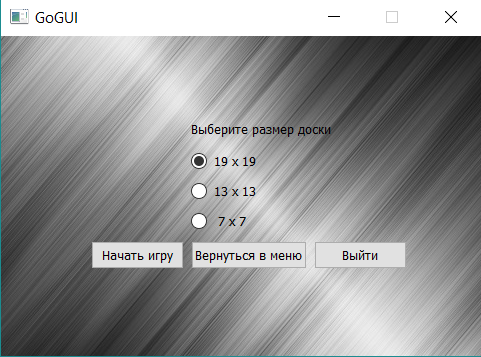
\includegraphics[scale=0.6]{pics/GoGUI/Settings.png}
	    \caption{Предыгровые настройки} 
		\label{pic:CUI_Settings}
	\end{center}
\end{figure}

\begin{figure}[H]
	\begin{center}
		
\includegraphics[scale=0.5]{pics/GoGUI/Game.png}
	    \caption{Окно игрового процесса} 
		\label{pic:CUI_Game}
	\end{center}
\end{figure}

\section*{Процесс обеспечения качества и тестирование}
\addcontentsline{toc}{section}{Глава 4. Процесс обеспечения качества и тестирование}

%Глава -- "Процесс обеспечения качества и тестирование". Здесь описываете процесс разработки -- количество ревью (и примерное количество %замечаний), количество демонстраций (с указанием конкретных замечаний и комментариями по ним), список использованных утилит (cppcheck, %valgrind, gcov и т.д, кто пользовался jenkins -- про него тоже) с комментариями как и когда они помогали. Рассказать про автоматические %тесты (модульные, функциональные), про тестовые сценарии, которые они покрывают, процент покрытия. Рассказать про тестовые сценарии для %ручных тестов.

Разработка велась в цикле непрерывной интеграции при помощи jenkins, и она сопровождалась модульным и функциональным тестированием, статическим и динамическим анализом кода, ревью кода и демонстрациями.

\subsection*{Непрерывная интеграция}
	Непрерывная интеграция была осуществлена при помощи приложения jenkins, установленного на сервер с операционной системой Ubuntu. В цикле ci производилась сборка приложения 64-битным компилятором GCC, автоматически генерировалась doxygen документация к коду. Код анализировался статическим анализатором cppcheck и динамическим анализатором valgrind, которыми было выявлено множество стилевых и не только деффектов кода. Valgrind помогал находить утечки памяти. Помимо этого, jenkins запускал модульные и функциональные тесты и в виде графиков представлял информацию об их прохождении и провалах.
	
\subsection*{Тестирование}
Разработка велась таким образом, что под практически все методы всех классов движка предварительно писались модульные тесты. Это помогло избежать непредсказуемого поведения приложения и прочих ошибок. Затем, с помощью функциональных тестов тестировлись функциональности, и в приложение попадали уже прошедшие проверку на прочность функциональности.

\subsection*{Ревью}

Автор попросил всего лишь однажды сделать ему ревью кода. Было выявлено 73 замечания, с большей частью из которых автор согласен и постепенно исправляет деффекты кода, на которые указывают эти замечания.

Небольшое число ревью сказалось на качестве кода.

\subsection*{Демо}

\begin{enumerate}

\item Консоль. Отрисовка доски.

\item Консоль. Игровой процесс без интерактивной доски: она отрисовывается, но не в текущем состоянии.

Комментарии участников демо

\begin{itemize}
	\item В конце игры хочется узнать, кто победитель(некоторое сообщение в конце). Если требуется подсчитать очки, сказать, что пользователи должны посчитать очки.
	\item Добавить Help
\end{itemize}

\item Консоль. Игровой процесс с интерактивной отрисовкой доски, хелпом.

Комментарии участников демо

\begin{itemize}
	\item Добавить возможность начать игру заново.
	\item Выводить сообщение с подсказкой при неверном вводе.
	\item В конце игры выводить сообщение об окончании и предлагать начать заново.
\end{itemize}

\end{enumerate}

Все комментарии и пожелания участников демо я принял и реализовал. Они, объективно, сделали приложение лучше.

\section*{Выводы}
\addcontentsline{toc}{section}{Глава 5. Выводы}

%своими словами, с душой, от чистого сердца рассказать, чему удалось научиться за семестр, что извлечь.
За семестр были получены первые навыки объекто-ориентированного проектирования приложений на языке c++. Автор усвоил множество советов С. Мейерса по эффективному программированию на c++ и эффективному использованию STL и множество советов безопасного кодинга на c++. Был получен опыт от использования непрерывной интеграции. Автор познакомился со скриптовым языком bash для настройки непрерывной интеграции. Впервые было разработано приложение с графическим интерфесом.

К сожалению, в связи с тем, что для усвоения нового сложного материала понадобилось больше времени, чем было задумано, автор успел не в полной мере реализовать изначально задуманный проект. Автор собирается расширить функциональность движка, добавив, съедение камней и подсчет очков, а также ставит цель перед собой доделать приложение с графическим интерфейсом. Разработка простой базы данных для сохранения и загрузки процесса игры имеет меньший приоритет, чем ранее обозначенные задачи, но тем не менее планируется ее реализовать.

Итак, несмотря на то, что автор не успел реализовать все задумки, был получен большой опыт. Задачи обозначены, приоритеты расставлены. Планируется реализовать все задумки.


\section*{Приложения}
\addcontentsline{toc}{section}{Приложения}

\subsection*{Приложение 1. Листинги кода}
\addcontentsline{toc}{subsection}{Приложение 1. Листинги кода}

\subsubsection*{GoEngine}

\begin{itemize}
\item\textbf{GoEngineInterface}
\captionof{lstlisting}{GoEngineInterface.h}
\lstinputlisting[label=code:GoEngineInterface]{../../sources/GoEngine/GoEngineInterface.h}
\parindent=1cm % командна \lstinputlisting сбивает параментры отступа

\item\textbf{GoEngineAPI}
\captionof{lstlisting}{GoEngineAPI.h}
\lstinputlisting[label=code:GoEngineAPI.h]{../../sources/GoEngine/GoEngineAPI.h}
\parindent=1cm % командна \lstinputlisting сбивает параментры отступа

\captionof{lstlisting}{GoEngineAPI.cpp}
\lstinputlisting[label=code:GoEngineAPI.cpp]{../../sources/GoEngine/GoEngineAPI.cpp}
\parindent=1cm % командна \lstinputlisting сбивает параментры отступа

\item\textbf{Stone}
\captionof{lstlisting}{Stone.h}
\lstinputlisting[label=code:Stone.h]{../../sources/GoEngine/Model/Stone.h}
\parindent=1cm % командна \lstinputlisting сбивает параментры отступа

\captionof{lstlisting}{Stone.cpp}
\lstinputlisting[label=code:Stone.cpp]{../../sources/GoEngine/Model/Stone.cpp}
\parindent=1cm % командна \lstinputlisting сбивает параментры отступа

\item\textbf{Point}
\captionof{lstlisting}{Point.h}
\lstinputlisting[label=code:Point.h]{../../sources/GoEngine/Model/Point.h}
\parindent=1cm % командна \lstinputlisting сбивает параментры отступа

\captionof{lstlisting}{Point.cpp}
\lstinputlisting[label=code:Point.cpp]{../../sources/GoEngine/Model/Point.cpp}
\parindent=1cm % командна \lstinputlisting сбивает параментры отступа

\item\textbf{Board}
\captionof{lstlisting}{Board.h}
\lstinputlisting[label=code:Board.h]{../../sources/GoEngine/Model/Board.h}
\parindent=1cm % командна \lstinputlisting сбивает параментры отступа

\captionof{lstlisting}{Board.cpp}
\lstinputlisting[label=code:Board.cpp]{../../sources/GoEngine/Model/Board.cpp}
\parindent=1cm % командна \lstinputlisting сбивает параментры отступа

\item\textbf{Move}
\captionof{lstlisting}{Move.h}
\lstinputlisting[label=code:Move.h]{../../sources/GoEngine/Rules/Move.h}
\parindent=1cm % командна \lstinputlisting сбивает параментры отступа

\captionof{lstlisting}{Move.cpp}
\lstinputlisting[label=code:Move.cpp]{../../sources/GoEngine/Rules/Move.cpp}
\parindent=1cm % командна \lstinputlisting сбивает параментры отступа

\item\textbf{GameProcess}
\captionof{lstlisting}{GameProcess.h}
\lstinputlisting[label=code:GameProcess.h]{../../sources/GoEngine/Rules/GameProcess.h}
\parindent=1cm % командна \lstinputlisting сбивает параментры отступа

\captionof{lstlisting}{GameProcess.cpp}
\lstinputlisting[label=code:GameProcess.h]{../../sources/GoEngine/Rules/GameProcess.cpp}
\parindent=1cm % командна \lstinputlisting сбивает параментры отступа

\item\textbf{Exceptions}
\captionof{lstlisting}{IncorrectDiagonalException.h}
\lstinputlisting[label=code:IncorrectDiagonalException]{../../sources/GoEngine/Model/Exceptions/IncorrectDiagonalException.h}
\parindent=1cm % командна \lstinputlisting сбивает параментры отступа

\captionof{lstlisting}{MoveException.h}
\lstinputlisting[label=code:MoveException]{../../sources/GoEngine/Rules/Exceptions/MoveException.h}
\parindent=1cm % командна \lstinputlisting сбивает параментры отступа

\captionof{lstlisting}{MoveOutsideTheBoardException.h}
\lstinputlisting[label=code:MoveOutsideTheBoardException]{../../sources/GoEngine/Rules/Exceptions/MoveOutsideTheBoardException.h}
\parindent=1cm % командна \lstinputlisting сбивает параментры отступа

\captionof{lstlisting}{MoveRepeatException.h}
\lstinputlisting[label=code:MoveRepeatException]{../../sources/GoEngine/Rules/Exceptions/MoveRepeatException.h}
\parindent=1cm % командна \lstinputlisting сбивает параментры отступа

\captionof{lstlisting}{MoveToDieException.h}
\lstinputlisting[label=code:MoveToDieException]{../../sources/GoEngine/Rules/Exceptions/MoveToDieException.h}
\parindent=1cm % командна \lstinputlisting сбивает параментры отступа

\captionof{lstlisting}{MoveToNotEmtyPointException.h}
\lstinputlisting[label=code:MoveToNotEmtyPointException]{../../sources/GoEngine/Rules/Exceptions/MoveToNotEmtyPointException.h}
\parindent=1cm % командна \lstinputlisting сбивает параментры отступа

\end{itemize}

\subsection*{Приложение 2. Doxygen документация}
\addcontentsline{toc}{subsection}{Приложение 2. Doxygen документация}



%\subsection*{Частичный листинг}
%% настрока частичного ввода (требуется один раз)
%\makeatletter
%\def\lst@PlaceNumber{\llap{\normalfont
%                \lst@numberstyle{\the\lst@lineno}\kern\lst@numbersep}}
%\makeatother

%\captionof{lstlisting}{фрагмент hell\_o.c}
%\lstinputlisting[label=code:hello_mod, linerange={4-5}]{listings/hell_o.c}
%\parindent=1cm

%\subsection*{Таблица}

%\begin{table}[H]
%	\begin{center}
%		\begin{tabular}{|l|l|}
%			\hline
%			top left & top right\\ \hline
%			bot left & bot right\\ \hline
%		\end{tabular}
%		\caption{ Название таблицы}
%		\label{tabular:tab_examp}
%	\end{center}
%\end{table}
\end{document}
